%!TEX root = ../main.tex

Sea $M$ un espacio topologico y denotemos el espacio
$$M^n=M\times M\times\dots\times M,$$
para $n\geq 1$, con la topologia producto.
\begin{definition}
    El subespacio de $M^n$ definido como
    $$\mathcal{F}_n(M):=\{(u_1,\ldots,u_n)\in M^n|u_i\neq u_j\text{ para todo }i\neq j\},$$
    se conoce como el \textit{espacio de configuracion} de $n-$tuplas ordenadas de puntos en $M.$
\end{definition} 
\begin{eg}
    Si bien es practicamente imposible visualizar este espacio para casos de interes podemos dar representaciones esquematicas de que es un punto. Por ejemplo el punto $((1,0),(2,0))\in \mathcal{F}_2(\R^2)$ es
    \begin{center}
        

\tikzset{every picture/.style={line width=0.75pt}} %set default line width to 0.75pt        

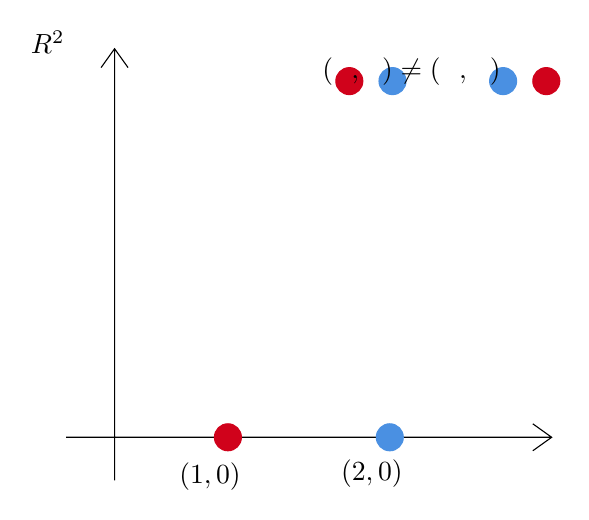
\begin{tikzpicture}[x=0.75pt,y=0.75pt,yscale=-1.3,xscale=1.3]
%uncomment if require: \path (0,877); %set diagram left start at 0, and has height of 877

%Shape: Axis 2D [id:dp8161459569391534] 
\draw  (150,194) -- (330,194)(168,50) -- (168,210) (323,189) -- (330,194) -- (323,199) (163,57) -- (168,50) -- (173,57)  ;
%Shape: Circle [id:dp3879912667843207] 
\draw  [color={rgb, 255:red, 208; green, 2; blue, 27 }  ,draw opacity=1 ][fill={rgb, 255:red, 208; green, 2; blue, 27 }  ,fill opacity=1 ] (205,194) .. controls (205,191.24) and (207.24,189) .. (210,189) .. controls (212.76,189) and (215,191.24) .. (215,194) .. controls (215,196.76) and (212.76,199) .. (210,199) .. controls (207.24,199) and (205,196.76) .. (205,194) -- cycle ;
%Shape: Circle [id:dp27918612907050666] 
\draw  [color={rgb, 255:red, 74; green, 144; blue, 226 }  ,draw opacity=1 ][fill={rgb, 255:red, 74; green, 144; blue, 226 }  ,fill opacity=1 ] (265,194) .. controls (265,191.24) and (267.24,189) .. (270,189) .. controls (272.76,189) and (275,191.24) .. (275,194) .. controls (275,196.76) and (272.76,199) .. (270,199) .. controls (267.24,199) and (265,196.76) .. (265,194) -- cycle ;
%Shape: Circle [id:dp8020177018586152] 
\draw  [color={rgb, 255:red, 208; green, 2; blue, 27 }  ,draw opacity=1 ][fill={rgb, 255:red, 208; green, 2; blue, 27 }  ,fill opacity=1 ] (250,62) .. controls (250,59.24) and (252.24,57) .. (255,57) .. controls (257.76,57) and (260,59.24) .. (260,62) .. controls (260,64.76) and (257.76,67) .. (255,67) .. controls (252.24,67) and (250,64.76) .. (250,62) -- cycle ;
%Shape: Circle [id:dp7823010661440502] 
\draw  [color={rgb, 255:red, 208; green, 2; blue, 27 }  ,draw opacity=1 ][fill={rgb, 255:red, 208; green, 2; blue, 27 }  ,fill opacity=1 ] (323,62) .. controls (323,59.24) and (325.24,57) .. (328,57) .. controls (330.76,57) and (333,59.24) .. (333,62) .. controls (333,64.76) and (330.76,67) .. (328,67) .. controls (325.24,67) and (323,64.76) .. (323,62) -- cycle ;
%Shape: Circle [id:dp2546903353916321] 
\draw  [color={rgb, 255:red, 74; green, 144; blue, 226 }  ,draw opacity=1 ][fill={rgb, 255:red, 74; green, 144; blue, 226 }  ,fill opacity=1 ] (266,62) .. controls (266,59.24) and (268.24,57) .. (271,57) .. controls (273.76,57) and (276,59.24) .. (276,62) .. controls (276,64.76) and (273.76,67) .. (271,67) .. controls (268.24,67) and (266,64.76) .. (266,62) -- cycle ;
%Shape: Circle [id:dp5671014248101258] 
\draw  [color={rgb, 255:red, 74; green, 144; blue, 226 }  ,draw opacity=1 ][fill={rgb, 255:red, 74; green, 144; blue, 226 }  ,fill opacity=1 ] (307,62) .. controls (307,59.24) and (309.24,57) .. (312,57) .. controls (314.76,57) and (317,59.24) .. (317,62) .. controls (317,64.76) and (314.76,67) .. (312,67) .. controls (309.24,67) and (307,64.76) .. (307,62) -- cycle ;

% Text Node
\draw (191,202.4) node [anchor=north west][inner sep=0.75pt]    {$( 1,0)$};
% Text Node
\draw (251,201.4) node [anchor=north west][inner sep=0.75pt]    {$( 2,0)$};
% Text Node
\draw (136,42.4) node [anchor=north west][inner sep=0.75pt]    {$\mathbb{R}^{2}$};
% Text Node
\draw (244,52.4) node [anchor=north west][inner sep=0.75pt]    {$( \ \ ,\ \ ) \neq ( \ \ ,\ \ )$};


\end{tikzpicture}
    \end{center}
    Note que tenemos que tener muy presente el orden de escogencia en el grafico, ya que si no podriamos confundir este punto con $((2,0),(1,0))$
\end{eg}
Con este espacio tenemos que
\begin{definition}
    El grupo fundamental $\pi_1(\mathcal{F}_n(M))$ se conoce como el \textit{grupo de trenzas puras} de $M$ en $n$ cuerdas.
\end{definition}

Posteriormente veremos cuando este es equivalente y algunas descripciones interesantes.